\documentclass[11pt,a4paper]{article}
\usepackage[utf8]{inputenc}
\usepackage{amsmath}
\usepackage{amssymb}
\usepackage{graphicx} 


\begin{document}
%%%%%%%%%%%%%%%%%%%%%%%%%%%%%%%%%%%%%%%%%%%%%%%%%%%%%%%%%%%%%%%%%%%
	\begin{figure}
  	\hspace*{-15.0mm} {
\includegraphics[width=50mm]{logo}}
  	\end{figure}
  
\hspace{10mm}
%%%%%%%%%%%%%%%%%%%%%%%%%%%%%%%%%%%%%%%%%%%%%%%%%%%%%%%%%%%%%%%%%%%
\begin{center}

\textit{\textbf{\Huge{ Studienmethodik und Selbstmanagement  SS 2015}}}\\
\emph{\textbf{1.Protokoll Gruppe 1} }
\begin{flushleft}
\textit{ Dozentin :  Antje Grießmayer }
\end{flushleft}

\end{center}
%%%%%%%%%%%%%%%%%%%%%%%%%%
\begin{flushright}
vom 23.03.2015
\end{flushright}
%%%%%%%%%%%%%%%%%%%%%%%%%%
\section*{Modulstermine}
\begin{enumerate}
\item Modul 23.03.15
\item Modul 20.04.15
\item Modul 04.05.15
\item Modul 18.05.15
\item Prüfung 15.06.15 um 11:00
\end{enumerate}

\section*{Referat}
\begin{itemize}
\item Der Vortrag  ist ca. 15 min
\item Alles mögliche benutzen (Beamer, ... )
\item Fragen stellen, interaktivsein und nicht nur Vorlesung halten.  
\end{itemize}
\textit{Die ersten drei Referate : basieren aufs Buch "Stephen R. Corey (7 Wege zu Effektivität)"}
\begin{itemize}
\item 1.Weg : Proaktivsein  (Vorträger LUKAS)
\item 2.Weg : Schon am Anfang der Sinn haben (Vorträger SIMON)
\item 3.Weg : Das wichtigste zuerst (Vorträger MICHAEL)
\end{itemize}

\section*{Feedback}
\begin{itemize}
\item Negativ bzw. positive das Referat beurteilen
\item Positiv zuerst (also was an dem Referat gut war ) dann negativ
\item Verbesserungen vorschlagen
\item Keine Verallgemeinerung (Was nicht gut an den Folien)
\item Ich -Botschaften formulieren 
\item konstruktiv sein
\item Danke sagt der Feedbackempfänger
\end{itemize}

\section*{Def. Studienmethodik}
  Eigene Lehrnarbeit koordinieren, um zum effektiven Lehrnen zu kommen. 
 \section*{Def. Selbstmanagment (Eisbergprinzip)}
Allgemeine Theorie der Persönlichkeit von  Freud  : was hindert mich etwas zu tun  
 
  	 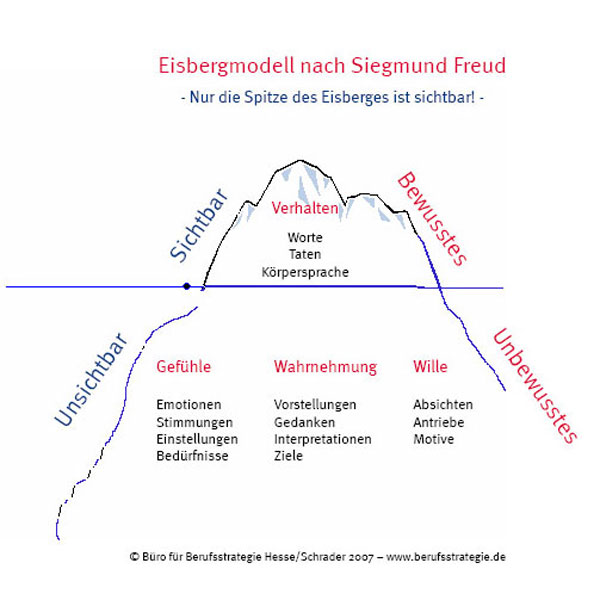
\includegraphics[width=100mm]{Eisbergprinzip}
  	 \begin{enumerate}
  	 \item Bewusstsein : 1/9 
  	 \item Unterbewusstsein : 8/9 \begin{itemize}
  	 \item Gefühle, Ängste, Instinkte, Wünsche nach Liebe, Bedürfnisse, Träume, Erfahrungen und Glaubensätze 
  	 \end{itemize}
  	 
  	 \end{enumerate}
  	 \section*{Verhältnismuster}
  Umsetzung der Glaubensätze : Warum verhält man sich so (z.B  Zurückhaltend, ..)
\section*{Arten von Protokollen}
\begin{enumerate}
\item Verlaufsprotokoll : allgemeines Protokollieren
\item Ergebnisprotokoll : Aufzählung von Resultaten mit einem Termin (in Unternehmen)\\
Wer macht was bis wann .
\item Fotoprotokoll : nicht mitschreiben sondern abfotografieren (ist simple)
\end{enumerate}

\section*{Zeitmanagment}
\begin{enumerate}
\item Erste Generation : \\ TO-DO Listen, Checklisten, Zeitplan, Wochenpläne und Kalender
\item Zweite Generation : \\ ( Eisenhauer) Prioritätssätze : Verschiedene Arten von Prioritäten 
\item Dritte Generation : \\ Wahrnehmung einer persönlichen Verantwortung im Einklang mit seinen Werten und Zielen
\end{enumerate}

\section*{Orientierung ans Modul}
\begin{itemize}
\item Volle Orientierung 
\item  Jeder von uns ist verantwortlich im Kurs und nicht nur die Dotzentin
\item Zuhören, Selbstverantwortung, Herzblut und Fragenstellen
\end{itemize} 

\end{document}
